% asset_id: AS2ModellingInMechanicsTIKZ-001
% lesson_id: AS2ModellingInMechanics
% related_svg: AS2ModellingInMechanicsSVG-001
% source: MechYr1-Chp8-Introduction.pdf, page 3
% related_section: Big Picture Explanation
% purpose: Show mechanics as the study of forces, motion, and the bridge F = ma.
\documentclass[tikz,border=8pt]{standalone}
\usepackage{amsmath}
\usetikzlibrary{arrows.meta, positioning, shapes.geometric}
\begin{document}
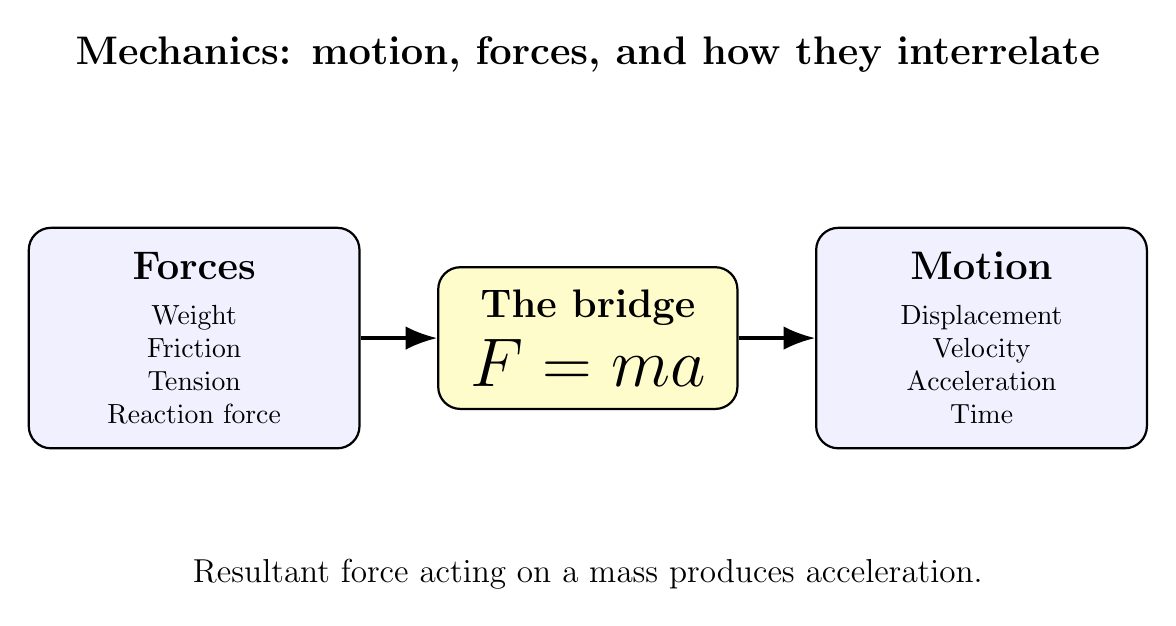
\begin{tikzpicture}[box/.style={draw, rounded corners=8pt, minimum width=4.2cm, minimum height=2.8cm, align=center, thick},bridge/.style={draw, rounded corners=8pt, minimum width=3.8cm, minimum height=1.8cm, align=center, thick},arrow/.style={-{Latex[length=4mm]}, very thick}]
\node[font=\Large\bfseries] at (0,3.6) {Mechanics: motion, forces, and how they interrelate};
\node[box, fill=blue!6] (forces) at (-5,0) {\Large\textbf{Forces}\\[4pt]Weight\\Friction\\Tension\\Reaction force};
\node[bridge, fill=yellow!20] (fma) at (0,0) {\Large\textbf{The bridge}\\[4pt]\Huge $F=ma$};
\node[box, fill=blue!6] (motion) at (5,0) {\Large\textbf{Motion}\\[4pt]Displacement\\Velocity\\Acceleration\\Time};
\draw[arrow] (forces.east) -- (fma.west);\draw[arrow] (fma.east) -- (motion.west);
\node[align=center, font=\large] at (0,-3.0) {Resultant force acting on a mass produces acceleration.};
\end{tikzpicture}
\end{document}
